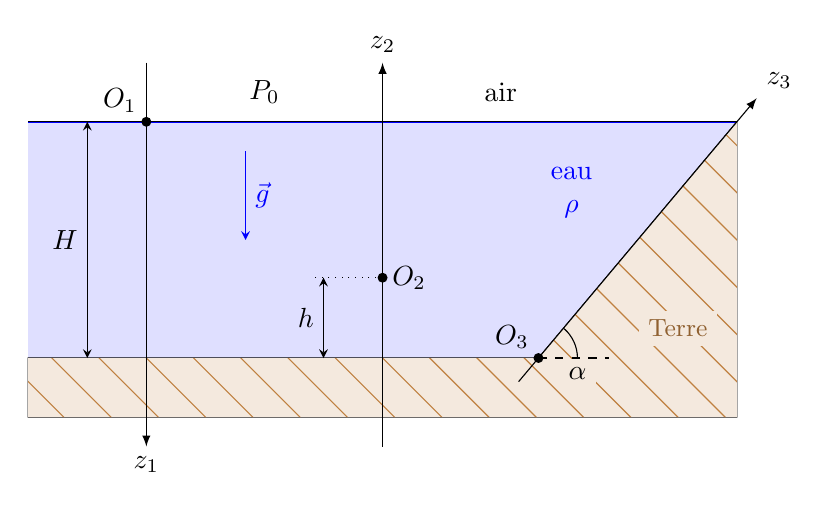
\begin{tikzpicture}[scale=1.5]
\begin{scope}
\draw[clip] (-1,0) rectangle(5,-2);
\fill[fill=blue!12.5!white] (-1,0) rectangle(5,-2);
\draw[very thin,blue](-1,0) -- (5,0);
\draw  (3.6,-0.6) node[blue,text centered, text width = 0.8cm]{eau  $\rho$};
\end{scope}

\begin{scope}
\draw[clip] (-1,-2.5) -- (-1,-2) -- (3.32,-2) -- (5,0) -- (5,-2.5) -- cycle;
\fill[brown!17.5!white] (-1,-2.5) -- (-1,-2) -- (3.32,-2) -- (5,0) -- (5,-2.5) -- cycle;
\foreach \x in {-4,-3.6,...,5}{
	\draw[brown] (\x,0) -- +(-45:5);
}
\draw[brown!75!black] (4.5,-1.75) node[fill=brown!17.5!white]{\small Terre};
\end{scope}


%%%%%%%%%%% définition des axes
\draw[stealth-stealth] (-0.5,-2) -- +(0,2) node[midway,left]{$H$};
% ---------------    1
\draw[-latex] (0,0.5) -- +(0,-3.25) node[below]{$z_1$};
\fill (0,0) circle(1.2pt) node[above left]{$O_1$};
% ---------------    2
\draw[stealth-stealth] (1.5,-2) -- +(0,0.68) node[midway,left]{$h$};
\draw[-latex] (2,-2.75) -- +(0,3.25) node[above]{$z_2$};
\fill (2,-1.32) circle(1.2pt) node[right]{$O_2$};
\draw[dotted,thin] (2,-1.32) -- +(-0.6,0);
% ---------------    3
\draw[-latex] (3.152,-2.2) -- (5.168,0.2) node[above right]{$z_3$};
\fill (3.32,-2) circle(1.2pt) node[above left]{$O_3$};
\draw[dashed] (3.32,-2 ) -- +(0.6,0);
\draw (3.65,-2) node[fill=brown!17.5!white,below]{$\alpha$} arc(0:49:0.33);

\draw (1,0.25) node[]{$P_0$};
\draw (3,0.25) node[]{air};
\draw[-stealth,blue] (0.84,-0.25) -- +(0,-0.75) node[midway,right]{$\vec{g}$};
\end{tikzpicture}